\section{The Rust Model} \label{rust_model}

This section sets up the model whose input-output relationship I want to shed light on. I consider the single-agent dynamic discrete choice model of \citet{R87}. Every period an agent needs to decide whether to replace the engine of a bus in the carpark or to conduct standard maintenance operations. The Rust model assumes optimal behaviour of the agent and asks what the implied deep economic parameters are, given this optimal behaviour.

The model output I consider is implied annual demand for engine replacements. Model inputs are engine replacement costs and a cost parameter that is part of the agent’s utility function. In the Rust model these variables are estimated but I consider them to be inputs for the implied annual demand. Computing Shapley effects requires the simulation of the input variables. To that end, information about the distribution of the inputs are needed.

\subsection{Bus-Engine Replacement Model}

Information about the model is required for calculating the variance-covariance matrix and mean vector of the inputs.

In \citet{R87} an agent needs to manage a pool of buses for public transportation. Each period a bus exhibits an accumulated mileage state (odometer state) $x$ and other state variables $\varepsilon$, that are unobserved by the econometrician. The agent has to decide whether to perform standard maintenance or an expensive engine replacement. The agent’s decision in period $t$ is
\begin{equation}
i_t\ =
\begin{cases}
0,\ standard\ maintenance \\
1,\ replace\ engine.
\end{cases}
\end{equation}

\noindent If replacement is chosen, the accumulated mileage state $x$ is set to zero. Otherwise, the bus is used for another period with standard maintenance and $x$ increases until the next period. Note that $x$ needs to me discretised for the estimation. I follow \citet{R87} and discretise the state space into 175 grids with a size of each bin of 2,571 miles.

The agent’s utility function given state $(x, \varepsilon)$ is described by
\begin{equation}
u(x,\ i,\ \varepsilon;\ \theta_1,\ RC)=v(x,\ i;\ \theta_1,\ RC)+\varepsilon(i),
\end{equation}

where
\begin{equation*}
v(x,\ i;\ \theta_1,\ RC)=
\begin{cases}
-c(x; \theta_1),\ if\ d=0,\\
-RC-c(0;\theta_1),\ if\ d=1,
\end{cases}
\end{equation*}

\noindent and $\varepsilon(i)$ denotes utility shocks. In the above expression, $RC$ represents the expected replacement costs of an engine replacement, that is, net the possible payoff of selling the old engine. $c(x; \theta_1)$ is a cost function of operating a bus at state $x$. $\theta_1$ is a vector of structural parameters. I consider the linear cost function $c(x; \theta_{11}) = 0.001 \theta_{11} x$.

[Give intuition for what that means: utility depends on what? Give examples.]

How the state $(x, \varepsilon)$ changes over time, depends on the choice $i_t$ and is described by the Markovian transition density $p(x_{t+1}, \varepsilon_{t+1} \mid x_t, \varepsilon_t, i_t; \theta_2, \theta_3)$, where $\theta_2$ is assumed to be Euler’s constant and $\theta_3$ is a vector of transition probabilities. Markovian means that $p$ depends on $ (x_t, \varepsilon_t) $ only and not on other past states.

The discount factor is denoted $\beta \in (0,1) $. Given state $ (x_t,\ \varepsilon_t) $, the agent maximises, choosing a sequence of decisions
\begin{equation}
\max_{\{i_t,\ i_{t+1},\ i_{t+2},\ ...\}} E \left[\sum_{\tau=1}^\infty\ \beta^{\tau-t}\ u(x_{\tau},\ i_{\tau},\ \varepsilon_{\tau};\ \theta_1,\ RC) \right].
\end{equation}

By $p$ being Markovian, the optimal decision is time-invariant. Thus, drop time indices. The decision problem is now defined by the solution to the Bellman equation
\begin{multline}
V(x,\ \varepsilon)=\max_i \{ v(x,\ i;\ \theta_1,\ RC)+\varepsilon(i) + \\
\beta \int_{x'} \int_{\varepsilon'} V(x',\ \varepsilon')p(x',\ \varepsilon' \mid x,\ \varepsilon,\ i;\ \theta_2, \theta_3)dx' d \varepsilon' \}.
\end{multline}

The above problem is simplified by imposing some further assumptions to ease the estimation process. The model is solved by use of the so called NFXP \citep{R87}. The parameters to be estimated are combined in a vector $\theta=(\theta_3,\ RC,\ \theta_{11}) $. The estimation procedure via Maximum Likelihood is conducted by first estimating the transition probabilities $\theta_3$. In a second step, the parameters $RC$ and $\theta_{11}$ are estimated. I do not go into further details of how this model is solved. For details see \citet{R87}.

\subsection{Distribution of the Input Variables} \label{model_setup}

The Maximum Likelihood estimator is asymptotically normally distributed \citep{R73}. Thus, I estimate the variance-covariance matrix and the mean vector of $\theta_{11}$ and $RC$ by an MC simulation. Note that this general setup is used in \cref{comp_shap} as well. For solving the model, I use the simulation and estimation capabilities of the Python \textit{ruspy} package \citep{OSE19}. I chose \textit{scipy\_L-BFGS-B} as the solver for the NFXP algorithm \citep{SP20}. I proceed as follows.

First, I set the true parameters in $\theta$. I chose to consider three transition probabilities, i.e. the mileage state $x$ can increase from the current period to the next by two grids at most. I set
\begin{align*}
\theta_3 &= (\theta_{30},\ \theta_{31},\ \theta_{32})=(0.39189182,\ 0.59529371,\ 0.01281447),\\
RC &= 10.07780762,\\
\theta_{11} &= 2.29417622.
\end{align*}

\noindent Note that $RC$ is scaled by $0.001$ for estimation purposes. I consider a total of 50 buses for 120 periods (months, i.e. in total ten years).

\begin{table}
\centering
\caption{Variance-Covariance Matrix of the Input Variables}
\label{cov}
\begin{threeparttable}
\centering
\begin{tabular}{lrr}
\toprule
{} &      $RC$ &  $\theta_{11}$ \\
\midrule
$RC$          &  1.604736 &       0.605903 \\
$\theta_{11}$ &  0.605903 &       0.273094 \\
\bottomrule
\end{tabular}

\begin{tablenotes}
\small
\item \textit{Notes:} Estimated variance-covariance matrix based on $10,000$ samples.
\end{tablenotes}
\end{threeparttable}
\end{table}

\begin{figure}[t]
	\caption{Correlation Between the Input Variables}
    % \floatfoot{A note}
    \label{correlation}
	\vspace*{-4mm}
	\centering
	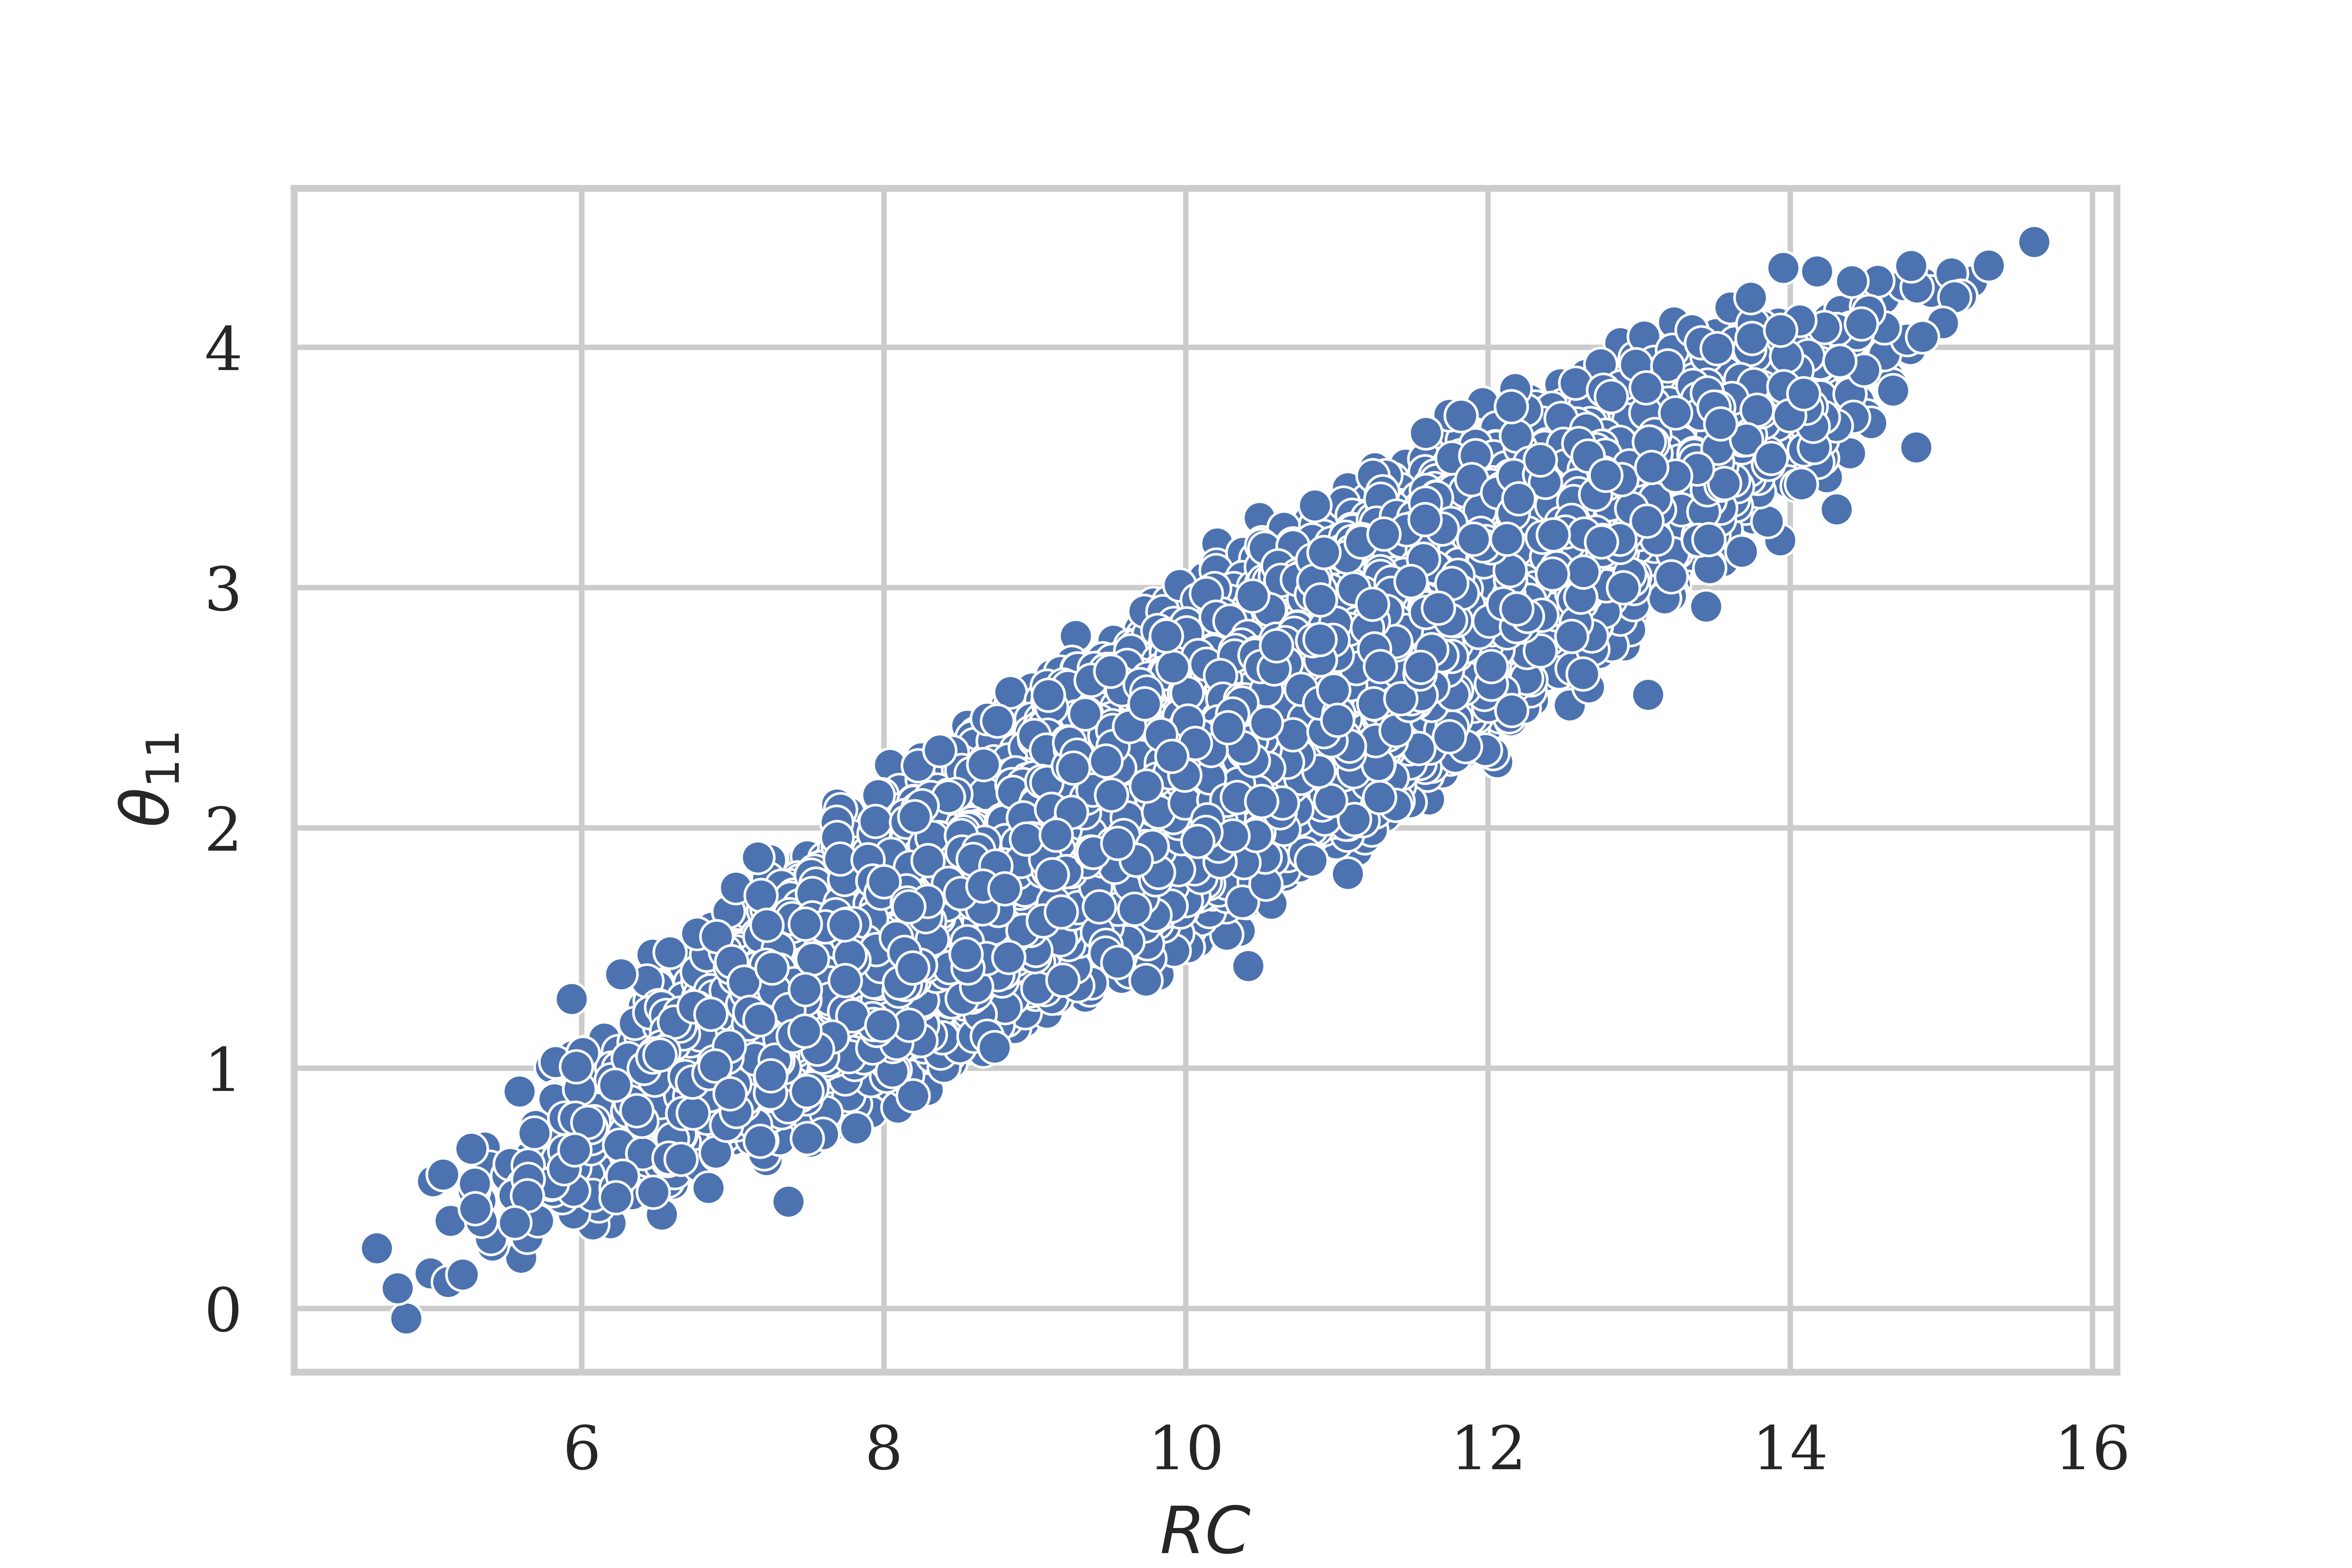
\includegraphics[scale=0.9]{../figures/correlation_rc_theta.png}
\end{figure}


Second, I simulate $10,000$ data sets from the above true parameters and estimate $\hat{\theta}, \hat{\theta}$ being the vector of estimated structural parameters.

Third, from the $10,000$ parameter estimates of $\widehat{RC}$ and ${\hat{\theta}}_{11}$, I calculate the sample variance-covariance matrix and the mean vector. \Cref{cov} shows the estimated variance-covariance matrix for $\widehat{RC}$ and ${\hat{\theta}}_{11}$. \Cref{cov} and \cref{correlation} show that $\widehat{RC}$ and ${\hat{\theta}}_{11}$ correlate, hinting that inputs in the Rust model are indeed dependent.

\subsection{Derivation of Implied Annual Demand}

\begin{figure}[t]
	\caption{Uncertainty Propagation}
    % \floatfoot{A note}
    \label{uncertainty}
	\vspace*{-4mm}
	\centering
	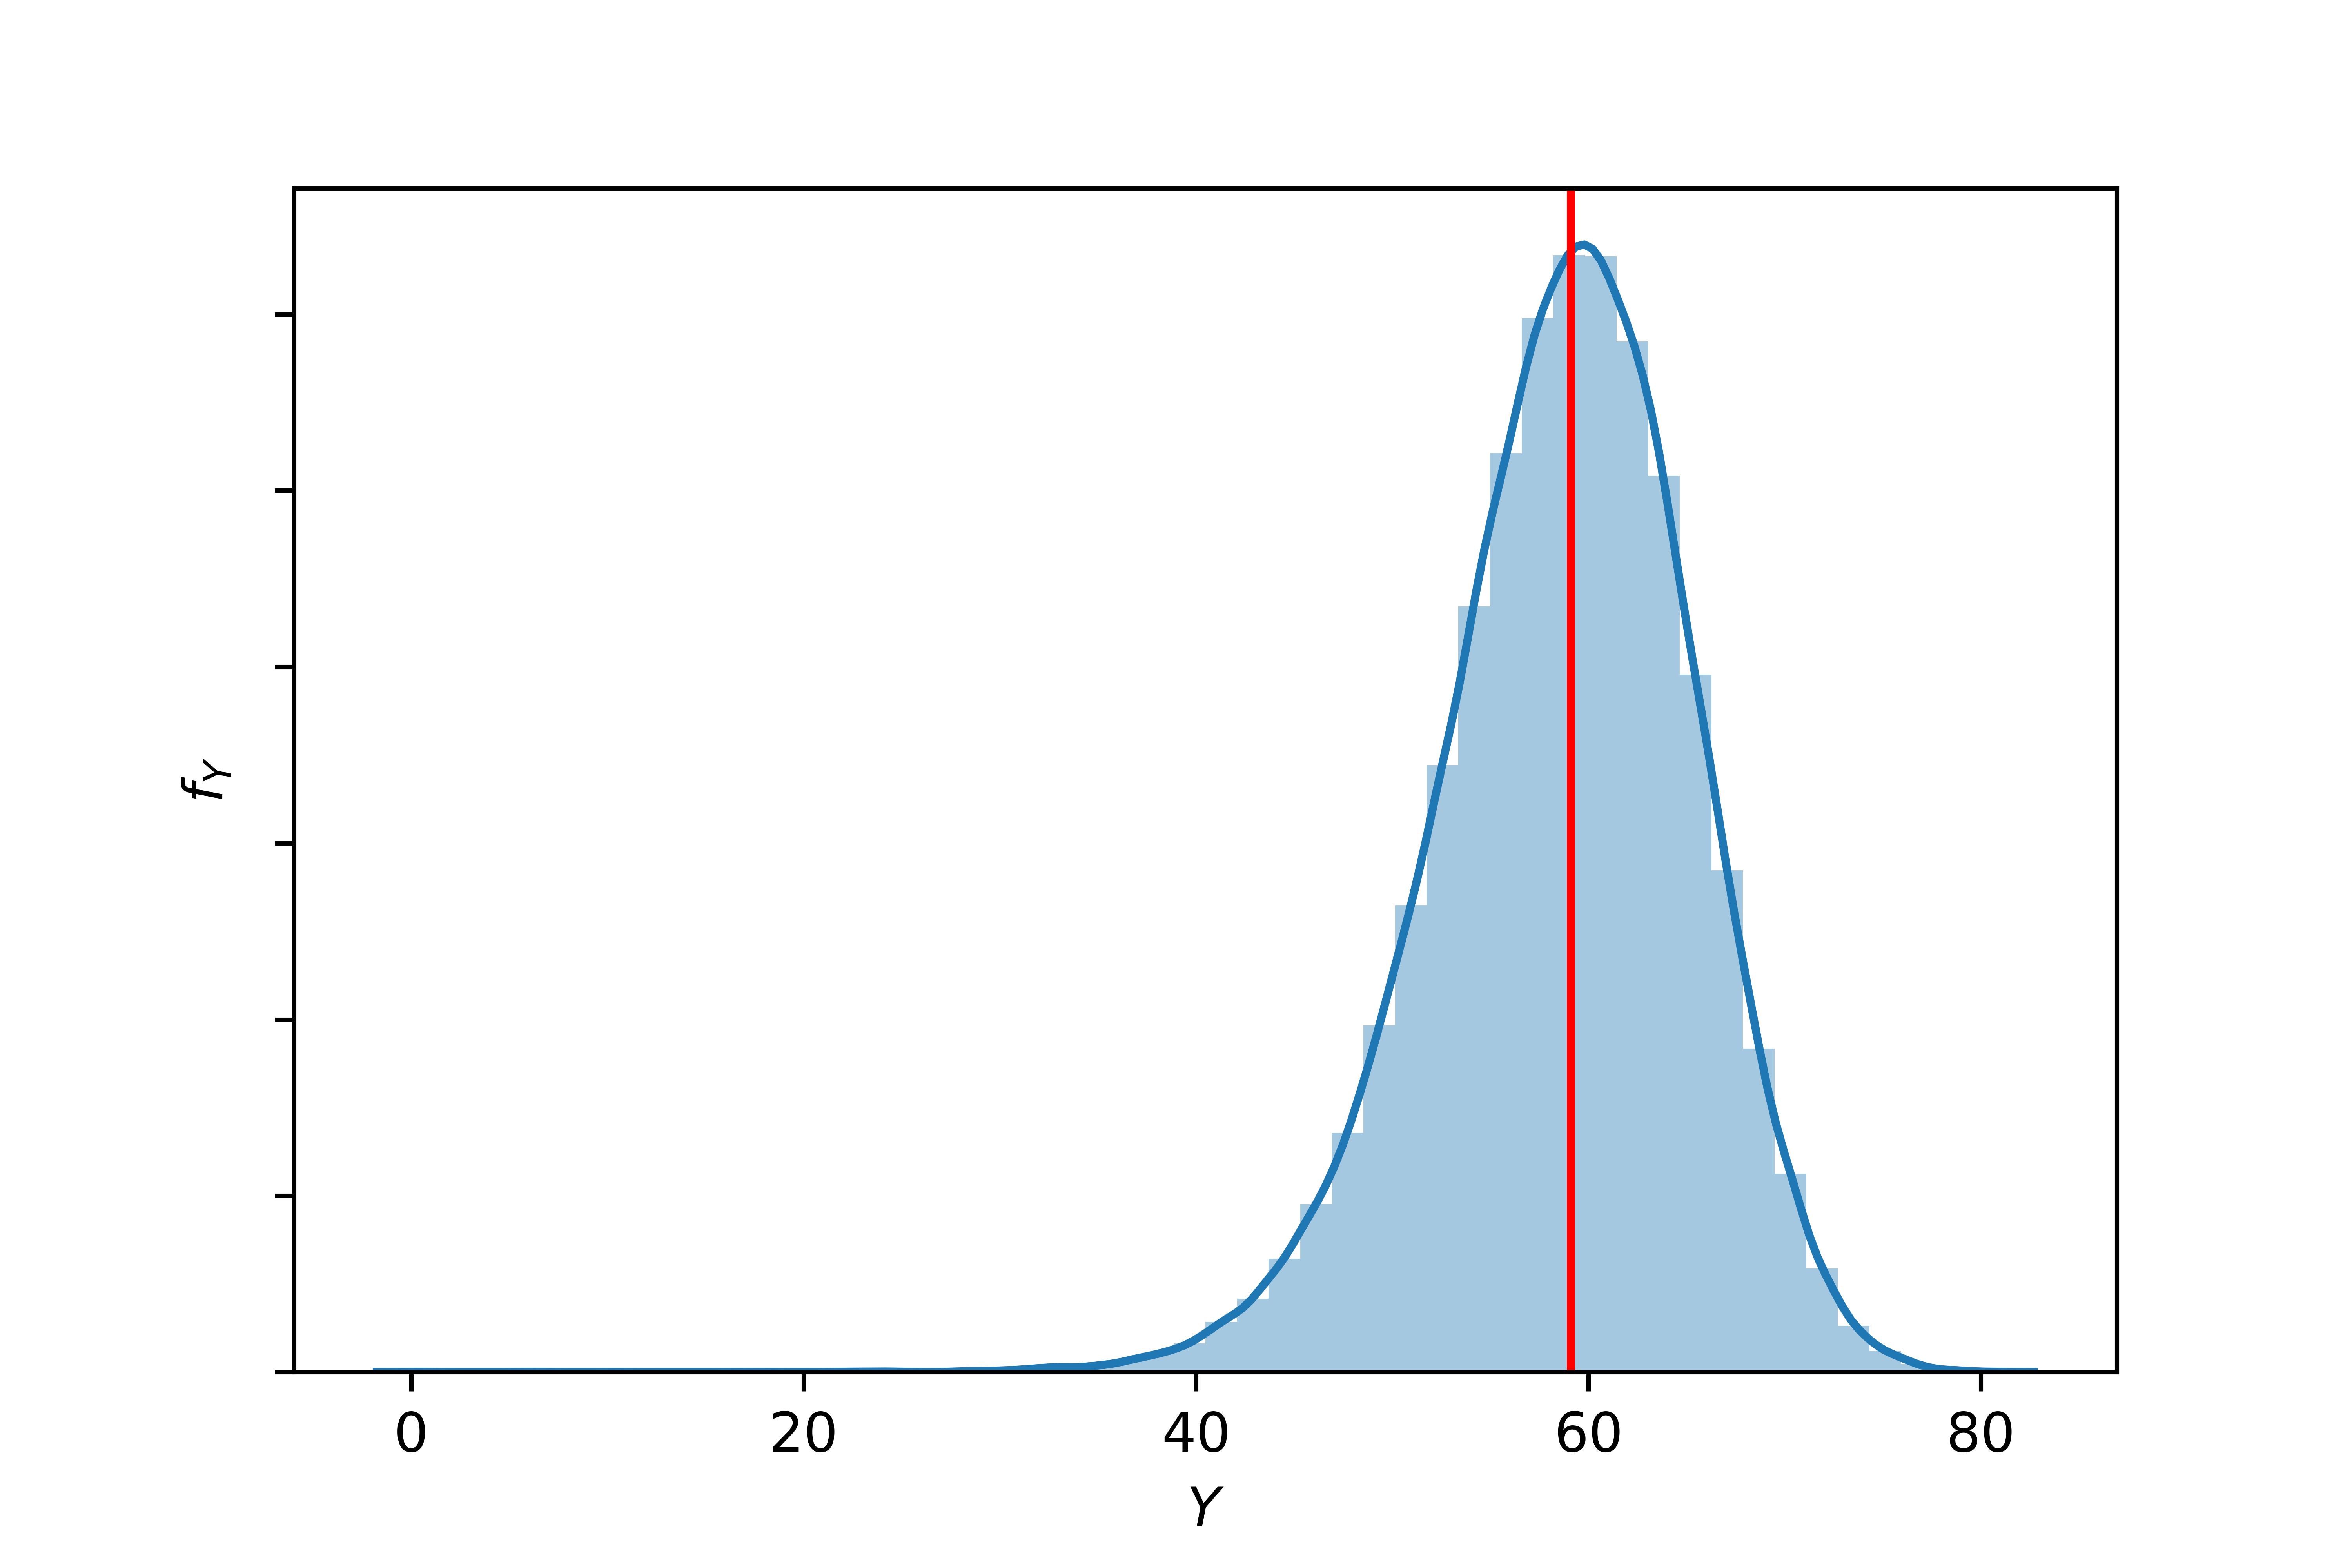
\includegraphics[scale=0.9]{../figures/uncertainty_propagation_100000.png}
\end{figure}

\citet{R87} shows how one can derive further quantities from the parameter estimates. \citet{R87} derives the implied annual demand (henceforth, demand) for bus-engine replacements. \citet{R87} computes the demand for bus engines by
\begin{equation}
\tilde{d}(RC)=\sum_{t=1}^{12}\ \sum_{i=1}^{M}\ {\tilde{i}}_t^m,
\end{equation}

\noindent where $M$ is the number of buses and ${\tilde{i}}_t^m$ is a realisation of the process $(i_t^m,\ x_t^m)$, with $m$ being the bus index. Here, $M=50$. Recall that a period is represented by one month, so we end up with the annual demand for 50 buses. $\tilde{d}(RC)$ is stochastic, since ${\tilde{i}}_t^m$ is. Let $\pi_m(x_0^m,\ i_0^m)$ denote the distribution of the initial state for each bus $m$. Given this, one can compute the probability distribution of $\tilde{d}(RC) $ by the transition probability $P(i_t \mid x_t,\ \theta)p(x_t \mid x_{t-1}, i_{t-1},\ \theta_3) $. Note that $P(\cdot)$ depends on $\theta$, i.e. it depends on $RC$ as well. We can compute demand for a range of values for $RC$. In my analysis I compute demand for a single value of $RC$ only; $RC^{demand}=11.5$, i.e. 11,500 money units. \citet{R87} considers the expected demand, i.e. $d(RC)=E[\tilde{d}(RC)]$. Assuming that the initial state distribution $\pi$ is the long-run equilibrium distribution of $(i_t,\ x_t)$, $\pi$ is the solution to
\begin{equation}
\pi(x,\ i)=\int_y \int_j P(i\ \mid\ x,\ \theta)\ p(x\ \mid\ y,\ \ j,\ \theta_3)\ \pi(dy,\ dj).
\end{equation}

Note, that $\pi$ is a function of $\theta$. Assuming further that the processes $ (i_t^m, x_t^m)$ and $(i_t^k, x_t^k)$ are independent for $k \neq m$, i.e. the process of a bus is independent from the process of any other bus, one can write
\begin{equation}
d(RC)=12 \cdot M \cdot \int_0^{\infty} \pi(dx,\ 1).
\end{equation}

To show how the uncertainty in the inputs $(RC, \theta_{11})$ propagate to the output, demand, see figure xy. I again use \textit{ruspy} for the computation of the demand at $RC^{demand}$. I compute demand for $100,000$ simulated data sets. The output is normally distributed as can be seen in figure xy with mean xx and variance xx.

Now, that the model, i.e. how the output depends on the inputs, has been clarified, one is ready to consider the computation of Shapley effects.
